\begin{statementbox}
\textbf{\textcolor{CStatement}{条件与核心换元}}
设 $t\in\mathbb R$、$t\ne0$。当正负同次幂成对出现时，令 $u=t+1/t$，则
\[
\boxed{u\in(-\infty,-2]\cup[2,+\infty)}.
\]
\begin{center}
\begin{tikzpicture}[font=\small]
\begin{axis}[width=12cm,height=5.7cm,axis lines=middle,
 xmin=-3.6,xmax=3.6,ymin=-4.5,ymax=4.5,
 xtick={-2,-1,1,2},ytick={-2,2},xlabel={$t$},ylabel={$u$},
 ylabel style={at={(axis description cs:0.5,1.1)},anchor=south},
 tick label style={font=\small},clip=false]
\addplot[CStatement,very thick,domain=0.24:3.5,samples=160] {x+1/x};
\addplot[CStatement,very thick,domain=-3.5:-0.24,samples=160] {x+1/x};
\addplot[CExample,only marks,mark size=2.5pt] coordinates {(1,2) (-1,-2)};
\addplot[CStatement,only marks] coordinates {(.5,2.5) (2,2.5)};
\draw[CStatement,densely dashed] (axis cs:.5,2.5)--(axis cs:2,2.5);
\node at (axis cs:-2.1,3.2) {$u=t+1/t$};
\node[anchor=south] at (axis cs:1.8,3.6) {$t=\frac12,2:\ u=\frac52$};
\end{axis}
\end{tikzpicture}

{\small 绿色点为边界 $(1,2)$、$(-1,-2)$；中间纵坐标 $(-2,2)$ 取不到。}
\end{center}

\[
\begin{aligned}
t^2+t^{-2}&=u^2-2,\\
t^3+t^{-3}&=u^3-3u,\\
t^4+t^{-4}&=u^4-4u^2+2.
\end{aligned}
\]
\textbf{\textcolor{CStatement}{首尾完整对称的四次方程}}（$a,b\in\mathbb R$）
\[
t^4+at^3+bt^2+at+1=0
\ \Longleftrightarrow\ u^2+au+b-2=0,
\]
其中须同时满足 $u=t+1/t$、$|u|\ge2$。常数项为 $1$，故 $t=0$ 不是根；除以 $t^2$ 后换元，筛选 $u$ 后还要解 $t^2-ut+1=0$。

\medskip
\textbf{\textcolor{CStatement}{另两种常用整体}}
令 $v=t-1/t\in\mathbb R$，则 $t^2+t^{-2}=v^2+2$、$t^3-t^{-3}=v^3+3v$。只含偶次倒数和时，也可令 $z=t^2+t^{-2}\ge2$。

\medskip
\textbf{\textcolor{CStatement}{通用递推}}
记 $S_n=t^n+t^{-n}$（整数 $n\ge0$），则 $S_0=2$、$S_1=u$，且
\[
\boxed{S_{n+1}=uS_n-S_{n-1}\qquad(n\ge1)}.
\]

\medskip
\textbf{\textcolor{CStatement}{拓展：正弦与余弦的整体换元（另一类题）}}
若题目反复出现 $\sin\theta+\cos\theta$ 和 $\sin\theta\cos\theta$，
可\textbf{另令} $t=\sin\theta+\cos\theta$，利用 $\sin^2\theta+\cos^2\theta=1$ 得
\[
\boxed{2\sin\theta\cos\theta=t^2-1},\qquad
\boxed{(1+\sin\theta)(1+\cos\theta)=\frac{(1+t)^2}{2}}.
\]
若 $0\le\theta\le\pi/2$，则 $1\le t\le\sqrt2$，等号 $t=\sqrt2$ 在
$\theta=\pi/4$ 时取得；若 $\theta$ 为任意实数，则 $-\sqrt2\le t\le\sqrt2$。
这里的 $t$ 是\textbf{另一道题中新设的整体变量}，不与上面的倒数式原变量混用。

\end{statementbox}
\clearpage

\begin{statementbox}
\textbf{\textcolor{CStatement}{拓展：指数函数的整体换元（直接设 $t=e^x+e^{-x}$）}}

设 $x\in\mathbb R$。因为 $e^x>0$、$e^{-x}=1/e^x$，两项互为倒数，故可直接令
\[
\boxed{t=e^x+e^{-x}\in[2,+\infty)}.
\]
这里的 $t$ 是指数题中的\textbf{新整体变量}，不是前面倒数型的原变量。$t=2$ 当且仅当 $x=0$。
\begin{center}
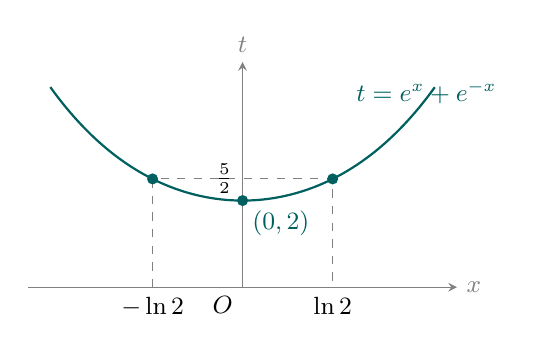
\begin{tikzpicture}[x=1.65cm,y=0.55cm,>=stealth, font=\small]
\draw[->,gray] (-1.65,0)--(1.65,0) node[right] {$x$};
\draw[->,gray] (0,0)--(0,5.2) node[above] {$t$};
\draw[teal!75!black,thick,domain=-1.48:1.48,samples=100] plot (\x,{exp(\x)+exp(-\x)});
\draw[dashed,gray] (-0.693,0)--(-0.693,2.5)--(0.693,2.5)--(0.693,0);
\fill[teal!75!black] (0,2) circle (2pt) node[below right] {$(0,2)$};
\fill[teal!75!black] (-0.693,2.5) circle (2pt);
\fill[teal!75!black] (0.693,2.5) circle (2pt);
\node[below] at (-0.693,0) {$-\ln2$};
\node[below] at (0.693,0) {$\ln2$};
\node[left] at (0,2.5) {$\frac52$};
\node[teal!75!black,anchor=west] at (0.8,4.5) {$t=e^x+e^{-x}$};
\node[below left] at (0,0) {$O$};
\end{tikzpicture}
\end{center}

\[
\boxed{\begin{aligned}
e^{2x}+e^{-2x}&=t^2-2,\\
e^{3x}+e^{-3x}&=t^3-3t,\\
e^{4x}+e^{-4x}&=t^4-4t^2+2,\\
(e^x-e^{-x})^2&=t^2-4.
\end{aligned}}
\]
任意整数 $n\ge0$，记 $A_n=e^{nx}+e^{-nx}$，则 $A_0=2$、$A_1=t$，且 $A_{n+1}=tA_n-A_{n-1}$（$n\ge1$）。

\textbf{回代：} 若 $t=c\ge2$，则
\[
\boxed{x=\ln\frac{c\pm\sqrt{c^2-4}}{2}}.
\]
当 $c=2$ 时只有 $x=0$；当 $c>2$ 时有两个互为相反数的解。若原题另有限制 $x$ 的范围，还要重新确定 $t$ 的范围并筛选回代结果。

\textbf{推广：} 将 $e$ 换成任意底数 $a>0$、$a\ne1$，直接令 $t=a^x+a^{-x}$，上述降次公式与范围仍成立；回代时把 $\ln$ 换成 $\log_a$。
\end{statementbox}
\clearpage
